\documentclass[
	oneside,
	parskip=half,
	% 10pt,
	a4paper,
]{scrbook}

\pdfcompresslevel=0
\pdfobjcompresslevel=0

\usepackage{xcolor}
\definecolor{seeblau}{HTML}{00A9E0}
\definecolor{seegrau}{HTML}{9AA0A7}

\definecolor{seeblau1}{HTML}{CCEEF9}
\definecolor{seeblau2}{HTML}{A6E1F4}
\definecolor{seeblau3}{HTML}{59C7EB}
\definecolor{seeblau4}{HTML}{00A9E0}
\definecolor{seeblau5}{HTML}{008ECE}


\usepackage{graphicx}
\usepackage{amsmath}
\usepackage{subcaption}
\usepackage{wrapfig}
\usepackage[english]{babel}
\usepackage{blindtext}
\usepackage{marginnote}
\usepackage{microtype}
\usepackage{siunitx}
\usepackage[utf8]{inputenc}
\usepackage{csquotes}
\usepackage{nicefrac}
\usepackage[T1]{fontenc}

\usepackage{siunitx}

% select serif font ###########################################################
% \usepackage[rm]{libertinus-type1}
% \usepackage{libertinus}
% \usepackage{roboto-serif}
\usepackage{libertinus}
% \usepackage[sfdefault, scaled=1.05]{biolinum}
% \usepackage{charter}	% designed for 300dpi print
% select sans serif font ######################################################
\usepackage{roboto}
% select math font ###########################################################
% \usepackage{newtxmath}
% \usepackage{sfmath} % sans serif math based on fira sans?
% \usepackage{eulervm}
% \usepackage[scaled=1.063]{libertinust1math}
% \usepackage{notomath}
% \usepackage{unicode-math}
\usepackage{amsfonts}
\usepackage{amssymb}
\usepackage{todonotes}


\setkomafont{disposition}{\normalfont\sffamily}

% not recommended with KOMA-script
\usepackage{tocloft}
\renewcommand\cftchappagefont{\normalfont}
\renewcommand\cftchapfont{\normalfont}
\renewcommand\cftchappresnum{\bfseries}
\renewcommand\cftchapaftersnum{}
\renewcommand{\cftchapfont}{\sffamily}
\renewcommand{\cftsecfont}{\sffamily}
\renewcommand{\cftsubsecfont}{\sffamily}
\renewcommand{\cftchappagefont}{\sffamily}
\renewcommand{\cftsecpagefont}{\sffamily}
\renewcommand{\cftsubsecpagefont}{\sffamily}

% caption
\usepackage{caption}
\captionsetup{
	% font={sf},
	labelfont={sf, bf, color=seeblau},
	labelsep=quad,
	labelformat=simple,
}

% links
\usepackage{hyperref}
\hypersetup{
	colorlinks=true,
	linkcolor=seeblau,
	citecolor=seeblau,
	urlcolor=seeblau,
	% hidelinks=true
}

% bibliography
\usepackage[
	style=numeric-comp, % comp = compressed 4,5,6,7 -> 4-7
	sorting=none,		% Sort by appearance
	% autocite = superscript,
	% backref=true,
	hyperref=true,
	url=true,
	maxbibnames=100
]{biblatex}
\addbibresource{../literature.bib}
\DefineBibliographyStrings{english}{%
    backrefpage  = {see p.}, % for single page number
    backrefpages = {see pp.} % for multiple page numbers
}

% remove issue
\AtEveryBibitem{%
  \clearfield{number}
}

\usepackage{float}
% \floatplacement{figure}{h}
% \floatplacement{table}{H}

% loosen float placement rules
\renewcommand{\topfraction}{0.8}
\renewcommand{\bottomfraction}{.8}
% \renewcommand{\textfraction}{0.1}
\renewcommand{\floatpagefraction}{.9}
% make floats less likely to be placed on a separate page
% \setcounter{totalnumber}{9}
% \setcounter{topnumber}{9}
% \setcounter{bottomnumber}{9}

% decrease space between floats and text
% \setlength{\textfloatsep}{0.5cm}
% \setlength{\floatsep}{0.5cm}
% % decrease space between figure and caption
% \setlength{\abovecaptionskip}{0.2cm}
% \setlength{\belowcaptionskip}{0.2cm}


\usepackage{adjustbox}

\usepackage{datetime}
\newdateformat{dotdate}{
	\twodigit{\THEDAY}.\twodigit{\THEMONTH}.\THEYEAR
}
\newdateformat{monthyeardate}{%
  \monthname[\THEMONTH] \THEYEAR}

% header and footer

\usepackage[
  markcase=noupper
]{scrlayer-scrpage}% activates pagestyle scrheadings automatically
\clearpairofpagestyles
\setkomafont{pageheadfoot}{\normalfont\sffamily}
\setkomafont{pagenumber}{\normalfont\sffamily}
\chead*{\color{seegrau} Draft \dotdate\today}
\ofoot*{\pagemark}
\ohead*{\rightmark}


\title{Optical signature of magnetic phase transition in transition metal phosphorus sulfides}
\subtitle{Bachelor Thesis}
\author{Leon Oleschko}

\begin{document}
\frontmatter
\begin{titlepage}
	% add university logos
	\begin{minipage}{.49\textwidth}
		\raggedright
		\includegraphics[height=20mm]{../figures/logo/UniWarsaw.png}
	\end{minipage}
	\begin{minipage}{.49\textwidth}
		\raggedleft
		\includegraphics[height=20mm]{../figures/logo/UniKonstanz_Logo.pdf}
	\end{minipage}

	\raggedright
	\sffamily

	\vspace{2cm}
	\newcommand{\markieren}[4]{
		\adjustbox{padding=3pt, bgcolor=seeblau1, margin=-1pt}{\strut{\sffamily\robotoMedium{#1}}}\\
		\adjustbox{padding=3pt, bgcolor=seeblau2, margin=-1pt}{\strut{\sffamily\robotoMedium{#2}}}\\
		\adjustbox{padding=3pt, bgcolor=seeblau3, margin=-1pt}{\strut{\sffamily\robotoMedium{#3}}}\\
		\adjustbox{padding=3pt, bgcolor=seeblau4, margin=-1pt}{\strut{\sffamily\robotoMedium{#4}}}
	}
	{
		\fontsize{32}{32}
		\markieren{Optical signature of}{magnetic phase transition}{in transition metal}{phosphorus sulfides}
	}

	\vspace{.25cm}
	{
		\Large
		Bachelor Thesis of Leon Oleschko\\
		\monthyeardate\today\\
	}
	
	\vfill
	\normalsize
	\raggedleft
	% \monthyeardate\today, 
	Fachbereich Physik, Universität Konstanz\\
	supervised by Dr. Mateusz Goryca,\\
	evaluated by Prof. Dr. Sebastian Gönnenwein

\end{titlepage}
{
	\sffamily
	\hypersetup{hidelinks}
	\tableofcontents
}
\clearpage

\section*{Summary}
Two-dimensional materials are of great interest due to their unique properties and potential applications in various fields, including nanocatalysis, optoelectronics, and spintronics \cite{MPX_review}. 
The selected van der Waals antiferromagnets NiPS$_3$, CrPS$_4$, MnPS$_3$ and FePS$_3$ are ideal candidates for the study of magnetic phase transitions with varying inter-layer coupling and exotic magnetic orders.
The materials can be easily exfoliated down to two-dimensional monolayers.\\
With bandgaps in the optical and near-infrared regions optical measurement techniques offer promising opportunities for fast in situ measurements of the magnetic structure on a limited probe volume.
Polarized photoluminescence has been identified as the most promising optical measurement techniques for studying the magnetic phase transition in the selected materials.\\
The magnetic splitting of the photoluminescence line of NiPS$_3$ has been demonstrated to be more interesting than previously thought, with different splitting observed for different linear polarization directions.\\
In CrPS$_4$ the circular dichroism ot the photoluminescence line is shown to be proportional to the magnetization, which allows the entire magnetic phase diagram to be studied with optical methods.

\vfill
\section*{Zusammenfassung}
Zweidimensionale Materialien erwecken aufgrund ihrer einzigartigen Eigenschaften und potenziellen Anwendungen in verschiedenen Bereichen wie der Nanokatalyse, der Optoelektronik und der Spintronik großes Interesse \cite{MPX_review}.
Die ausgewählten van-der-Waals Antiferromagnete NiPS$_3$, CrPS$_4$, MnPS$_3$ und FePS$_3$ sind ideale Kandidaten für die Untersuchung magnetischer Phasenübergänge mit unterschiedlicher interlayer-Kopplung und exotischen magnetischen Ordnungen.
Die Materialien lassen sich leicht auf zweidimensionale Monoschichten exfolieren.\\
Mit Bandlücken im optischen und nahinfraroten Bereich bieten optische Messmethoden vielversprechende Möglichkeiten für schnelle in-situ-Messungen der magnetischen Struktur in einem begrenzten Probenvolumen. 
Polarisierte Photolumineszenz wurde als vielversprechendste optische Messmethode zur Untersuchung des magnetischen Phasenübergangs in den ausgewählten Materialien identifiziert.\\
Die magnetische Aufspaltung der Photolumineszenzlinie von NiPS$_3$ hat sich als interessanter herausgestellt als bisher angenommen wurde, da für verschiedene lineare Polarisationen unterschiedliche Aufspaltungen beobachtet wurden.\\
In CrPS$_4$ wird gezeigt, dass der zirkuläre Dichroismus von der Photolumineszenzline proportional zur Magnetisierung ist, was es ermöglicht, das gesamte magnetische Phasendiagramm mit optischen Methoden zu untersuchen.

\vfill

\mainmatter

\chapter{Introduction}
\begin{wrapfigure}[13]{O}{.4\textwidth}
	\includegraphics[width=.4\textwidth]{../../figures/crystal structures/NiPS3 3d.png}\\
	\caption{NiPS$_3$ structure from \cite{NiPS3_coherent}}
	\label{fig:crystal structure}
\end{wrapfigure}
The interest in two-dimensional materials has grown due to their unique properties and potential applications in nanocatalysis, optoelectronics, and spintronics \cite{MPX_review}.

The class of \textit{transition metal phosphorus sulfides} offers a ideal combination of properties that make them an ideal subject for the study of two-dimensional materials.
These materials exhibit a wide range of exotic magnetic orders \cite{AFM_review}.

The crystal structure of one of the studied materials, NiPS$_3$, is illustrated in \autoref{fig:crystal structure}.
This structure is referred to as a \textit{van der Waals} layered material, as the material is highly anisotropic with quasi-2D layers held together by weak van der Waals forces.\\
The layers are easy to mechanically exfoliate, which allows the manufacture of samples with a thickness down to monolayers \cite{NiPS3_few_layer}.

Specifically, the materials NiPS$_3$, CrPS$_4$, MnPS$_3$, and FePS$_3$ were selected for measurements,  
as these materials exhibit a wide range of different magnetic behaviors, as the anisotropy of the magnetic interaction is different in each material \cite{MPS_magnetism,CrPS4_magnetic}.\\
The magnetic properties are dominated by the spins of the metal ions in the lattice \cite{MPS_magnetism, NiPS3_magnon_gap, CrPS4_magnetic}.\\
In NiPS$_3$ the interlayer coupling is weak and the spins of the Ni$^{2+}$ ions are in the layer planes \cite{MPS_magnetism}.\\
In contrast, to this, CrPS$_4$ exhibits strong interlayer coupling and has a magnetic structure that is perpendicular to the layers \cite{CrPS4_magnetic}.
The combination of this property together with easy exfoliation is promising, as it allows to alter the magnetic properties of the material.

The magnetic structure of all studied materials at low external magnetic field and below the Néel temperature of \SI{155}{K} for NiPS$_3$ and \SI{38}{K} for CrPS$_4$ \cite{MPS_magnetism, CrPS4_magnetic}  is anti-ferromagnetic.\\
In the anti-ferromagnetic phase, two sublattices align in opposite directions, resulting in a magnetization of $M=0$.\\
Over the Néel temperature, the magnetic order is paramagnetic with the spins randomly oriented and $M=0$.\\
When a sufficiently strong external magnetic field $H>H_\text{SF}$ is applied a \textit{magnetic phase transition} occurs, known as a spin-flop transition.
In this transition, all spins align with the magnetic field, resulting in a phase change from antiferromagnetic to ferromagnetic with $\vec{H}\propto \vec{M}>0$.\\
This happens for CrPS$_4$ at \SI{7.5}{T} \cite{CrPS4_magnetic} and for NiPS$_3$ at \SI{14}{T} \cite{NiPS3_magnon_gap}.
Unfortunately, the experimental capabilities were limited to \SI{10}{T}.

The selected materials offer useful optical properties, as they are semiconductors with a bandgap $E_B$ in the visible to near-infrared range.
Consequently, they are suitable for optical measurements.\\
Which have the advantage, that they can be used for fast, in situ measurements on a small sample volume or even with spatial resolution.\\
This allows the study of changes in the fast anti-ferromagnets through pump-probe or noise measurements \cite{AFM_review}.

The temporal resolution is constrained by the speed of the material-light interaction.\\
For an excitation photon to be absorbed by a semiconductor the photon energy $E_\text{ex} =h\nu= \nicefrac{hc}{\lambda}$ must exceed that of the bandgap $E_B$.
This results in the excitation of an electron $e^-$ from the valence band to the conduction band, accompanied by the creation of a hole $h^+$ in the valence band.\\
The electron and the hole can combine to form a neutral exciton $x$, a bound state of the electron and the hole, with a binding energy $E_x$.\\
Additionally, more complex structures such as charged excitons or biexcitons, can form with different binding energies.
All these structures can also be in excited states.\\
The energy difference $E_\text{ex}-E_B+E_x$ is dissipated through processes such as phonon emission, which heats the sample, intra-band photon emission, or a combination of these mechanisms.\\
The remaining energy is emitted as a luminescence photon with energy $E_B - E_x$, which can be observed as one strong peak in the spectrum for excitons and multiple smaller ones for the more complex structures.
\cite{MPX_first_principles,NiPS3_anisotropic,NiPS3_coherent,NiPS3_exciton}

When a local magnetic field $B=H+M$ is present, the luminescence line splits into two lines with different energies.
This phenomenon can be explained by the Zeeman effect or spin-orbit coupling of the exciton \cite{NiPS3_exciton}.\\
In addition, the bandgap also changes in response to the magnetic field \cite{MPS_magnetism}. 
This change can vary depending on the spin directions.
Therefore, changes for different circular polarizations can be expected \cite{MPX_first_principles}.\\
Various models have been proposed to explain the linear polarisation of the luminescence \cite{NiPS3_coherent, NiPS3_linear, NiPS3_exciton, NiPS3_anisotropic}.

The objective of this project is to identify optical signatures of the magnetic phase transition in the selected materials using a measurement technique that can be used for fast in situ measurements and on monolayers in the future.\\
This will enable further studies of the magnetic properties with temporal resolution through pump-probe or noise measurements, which is particularly relevant for spintronics applications \cite{AFM_review}.



\chapter{Methodology}
\section{Sample Preparation}
Prior to measurements, the samples have to be prepared.
The initial measurements were done on bulk crystals.
Subsequently, the samples were exfoliated, to expose a clean surface.
% \subsection*{Bulk Samples}
\begin{figure}
	\centering
	\begin{subfigure}[c]{.25\textwidth}
		\includegraphics[width=\textwidth]{../../photos/bulk_sample.jpg}
		\caption{Samples in \SI{2}{cm} vials.}
		\label{fig:samples_vials}
	\end{subfigure}
	\begin{subfigure}[c]{.25\textwidth}
		\includegraphics[width=\textwidth]{../figures/mounted_bulk_samples.jpg}
		\caption{Mounted bulk crystals. The crystals are under the black paper, glued to the copper holder.}	
		\label{fig:samples_bulk_mounted}
	\end{subfigure}
	\caption{Bulk Samples.}
\end{figure}
The bulk crystals were provided as shown in \autoref{fig:samples_vials}.
They were grown using the vapor transport method which is a conventional method for the manufacture of these materials \cite{review_tmd,AFM_review}.\\
The bulk crystals have dimensions of approximately $4 \times 2 \times \SI{.5}{mm}$.
The thickness was quantified using thin-film interference, as detailed in Section \ref{sec:thickness}.

For the initial measurements, the crystals were mounted to minimize strain below a piece of black paper with a hole that was glued to a holder on the corners as depicted in \autoref{fig:samples_bulk_mounted}.

\begin{figure}
	\centering
	\begin{subfigure}[t]{.25\textwidth}
		\includegraphics[width=\textwidth]{../../data/2023-11-02/i005_NiPS3_50x-scalebar.png}
		\caption{NiPS$_3$: Smooth surface with characteristic features from the hexagonal crystal lattice.}
		\label{fig:bulk_nips3}
	\end{subfigure}
	\begin{subfigure}[t]{.25\textwidth}
		\includegraphics[width=\textwidth]{../../data/2023-11-02/i009_FePS3_100x-scalebar.png}
		\caption{FePS$_3$: Rough surface.}
		\label{fig:bulk_feps3}
	\end{subfigure}
	\caption{Optical images of the bulk sample surface. Scalebar \SI{10}{\mu m}.}	
\end{figure}
Examined under a microscope the surface of NiPS$_3$, CrPS$_4$ and MnPS$_3$ samples was smooth like \autoref{fig:bulk_nips3} and the FePS$_3$ appeared rough like \autoref{fig:bulk_feps3}.\\
The surface appeared to be contaminated by a rough, oxidized layer. 
To remove this, mechanical exfoliation was used.


\subsection{Exfoliation}
\begin{figure}[h]
	\centering
	\begin{subfigure}[c]{.3\textwidth}
		\includegraphics[width=\textwidth]{../../photos/exfoliation.jpg}
		\caption{First Step: subdividing the crystal multiple times.}
		\label{fig:exfoliation_division}
	\end{subfigure}
	\begin{subfigure}[c]{.3\textwidth}
		\includegraphics[width=\textwidth]{../../photos/exfoliation glass.jpg}
		\caption{Second Step: transferring the flakes to a substrate.}
		\label{fig:exfoliation_transfer}
	\end{subfigure}
	\begin{subfigure}[c]{.3\textwidth}
		\includegraphics[width=\textwidth]{../../data/2023-12-04_LO_MG_NiPS3/CrPS4_50x_10um.png}\\
		\caption{Result: CrPS$_\text{4}$ flakes on Si/SiO$_\text{2}$ substrate, Scalebar 10$\mu$m}
		\label{fig:exfoliation_result}
	\end{subfigure}
	\caption{Exfoliation Process.}
	\label{fig:exfoliation}
\end{figure}
In order to prepare a surface that was free of contamination, particularly necessary on the FePS$_3$ crystals, mechanical exfoliation was used.
The stages of this process are photographed in \autoref{fig:exfoliation}.

Initially, a crystal with thickness $d_0$ is placed on an adhesive tape.\\
Subsequently, a second piece of tape is placed on top of the crystal and removed $n$ times.
This process is depicted in \autoref{fig:exfoliation_division}.
The flakes are divided each time into thinner flakes with the average thickness $\left< d_{n} \right> = \nicefrac{1}{2} \left< d_{n-1} \right>$.\\
For most samples $n$ was approximately $8$.
This technique allows to produce monolayers with $ \left<d_n\right>  = \SI{0.8}{nm}$ \cite{NiPS3_few_layer} from a $d_0 = \SI{400}{um}$ thick crystals, requiring just $n = \log_2 \nicefrac{d_0}{\left<d_n\right>} \approx 19$ steps.\\
The utilized adhesive tape is specially designed for exfoliation, although the use of a special adhesive tape is not necessary.
The main difference to normal \textit{commercial grade} adhesive tape is the availability of variants with different adhesive strengths 
and the tape material is flexible to prevent excessive pressure from being applied to the flake edges, thereby reducing the likelihood of breaking them.

Finally, the flakes are transferred to a substrate.
In \autoref{fig:exfoliation_transfer} the flakes are transferred to a glass substrate.
In this step, only the thinner flakes adhere to the substrate when the tape is removed, as they are more flexible and can better deform to the substrate.\\
The ratio of adhesion between the flakes and the substrate and the flakes and the tape determines the yield of flakes that remain on the substrate.\\
The adhesion between the flake and the substrate can be tuned by selecting different substrates.
For instance, the yield on glass was $10-100$ lower than on a Si/Si$_2$ substrate.
To alter the adhesion between the flakes and the tape, a different adhesive can be used. 
To get even more granularity the transfer was tried at elevated temperatures to reduce the adhesion.\\
To increase the yield even more this transfer step was repeated multiple times for the glass substrate.

The results are flakes on a substrate, as seen under a microscope in \autoref{fig:exfoliation_result}.
The resulting flakes have a thickness of approximately $\SI{500}{nm}$ and can be considered bulk material when compared to the thickness of monolayers.


\clearpage
\section{Measurement Techniques}
In order to identify the optical signatures of phase transitions, an optical measurement technique is used.
A few different methods were tried.

\begin{wrapfigure}[18]{O}{.4\textwidth}
	\includegraphics[width=.4\textwidth]{../figures/carray schematic.png}\\
	\caption\\
	Schematic of the transmission spectrometer from \cite{cary}.
	\label{fig:carry}
\end{wrapfigure}
\subsection{Transmission}
To measure a signal independently of the surface quality transmission spectroscopy can be used.
Specifically a commercial transmission spectrometer, the \textit{Cary 5000}, was utilized.
The schematic for it is shown in \autoref{fig:carry}.\\
\textit{Jan Suffczyński} was a great help in getting me up to speed with the machine and the cooling loop of the closed-cycle cryostat.

The functional principle is not explained in any of the provided documentation which would be interesting, because the spectrometer has surprisingly little noise.

The spectrometer has two user-accessible beam paths, one is the reference and one the sample.
A relative transmissivity is reported from the instrument, defined as $T = \nicefrac{T_\text{Sample}}{T_\text{Reference}}$.

\begin{figure}[b]
	\centering
	\includegraphics{../figures/2024-03-15 MnPS3 transmission raw.pdf}
	\caption{Raw data from the spectrometer.}
	\label{fig:transmission raw}
\end{figure}
For the initial measurements, MnPS$_3$ was selected because the \SI{.5}{mm} bulk crystals are already visually transparent.\\
The data is shown in \autoref{fig:transmission raw} for a MnPS$_3$ crystal in the sample path and for a hole in the sample path.

Surprisingly the relative transmission of the hole is not constant.\\
The only difference between the paths are the Quartz windows of the cryostat in which the sample was mounted and the aperture of the sample holder.
This does not explain the nonuniform transmission spectrum.\\
The machine changes from infrared to visible mode at \SI{800}{nm}, and there have been rumors that a technician from the company had serviced the machine and mixed up some filters.

Irrespective of the underlying cause, the measurement was reproducible and the signal can be corrected by dividing it with a calibration spectrum of the hole and aligning the visible and infrared spectra in software.

\begin{figure}
	\centering
	\includegraphics{../figures/2024-03-15 MnPS3 transmission processed.pdf }
	\caption{Corrected Absorption Signal of MnPS$_3$.}
	\label{fig:transmission corrected}
\end{figure}
The corrected absorption spectrum ($\approx 1 - T$) is depicted in \autoref{fig:transmission corrected} and reproduces the shape of the absorption spectrum in \cite{MnPS3_transmission}.
The bandgap is at \SI{2.6}{eV} above which the spectrometer saturates due to insufficient signal through the sample.

\begin{wrapfigure}[15]{O}{.3\textwidth}
	\includegraphics[width=.3\textwidth]{../../photos/transmission samples.jpg}
	\caption\\
	{Samples for Transmission Measurements.\\
	From left to right: FePS$_3$, NiPS$_3$ and CrPS$_4$.}
	\label{fig:transmission samples}
\end{wrapfigure}
\begin{figure}
	\centering
	\includegraphics{../figures/2024-03-15 Absorbance.pdf}
	\caption{Absorption Signal of different Samples.}
	\label{fig:transmission}
\end{figure}
For the other samples the features measured in \autoref{fig:transmission} correspond with those recorded in the literature \cite{CrPS4_transmission, NiPS3_transmission, FePS3_transmission}.

The main problem with this setup is that the spectrometer saturates quickly in the sample or the reference path when the sample is too thin or too thick.\\
It also has no way to individually display the intensity for the sample or reference path which makes adjustments difficult.

In order to obtain any usable measurements, the samples were exfoliated to a specific optical transparency, as shown in \autoref{fig:transmission samples}.
Additionally, a compensating aperture was placed in the reference beam.\\
To hold the thick exfoliated flakes they were not transferred to a substrate but mounted with the adhesive tape used for exfoliation. 
This method was successfully used down to \SI{10}{K} without any issues.

However, this workflow is rather tedious and there is no way to use a magnet with the spectrometer away.\\
It was planned to rebuild the transmission setup on the magnet, but this was not completed due to the time required for the unexpected measurements for Section \ref{sec:aligning flakes}.\\
Nevertheless, this technique remains promising as it allows for the independent measurement of the bandgap, circumventing luminescent phenomena.

\clearpage
\subsection{Reflection}
\begin{figure}
	\centering
	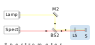
\includegraphics{../figures/setup_reflection.pdf}
	\caption{Setup used for reflection measurements.}
	\label{fig:reflection setup}
\end{figure}
Subsequently, reflection spectroscopy using the setup shown in \autoref{fig:reflection setup} was evaluated.\\
In this instance, a halogen lamp was utilized to illuminate the sample.
The light was focused by a lens (L$_5$) with a high numeric aperture on a small (in the order of \SI{10}{um}) spot.
The reflected beam passed through a beam-splitter (BS$_2$) into a spectrometer.\\
This technique only needs access to the sample from a single side, which simplifies the setup.

\begin{figure}
	\centering
	\includegraphics{../figures/2024-03-14 reflection spectra.pdf}
	\caption{Unprocessed reflection spectra from bulk crystals. With bandgap from transmission measurements.}
	\label{fig:reflection spectra}
\end{figure}
The unprocessed recorded spectra for bulk crystals of highly transparent MnPS$_3$ and the material with the strongest bandgap edge NiPS$_3$, are represented in \autoref{fig:reflection spectra}.\\
Below the bandgap, the crystals are transparent, and a thin-film interference pattern is visible.\\
Deconvolving the spectral shape of the lamp by dividing the signal from the sample with the spectrum of a mirror was attempted, but the objective lens L$_5$ in \autoref{fig:reflection setup} has a strong chromatic aberration, which alters the spectrum too much.

\begin{figure}
	\centering
	\includegraphics{../figures/2024-03-14 reflection spectra IMF.pdf}
	\caption{Filtered reflection spectra.}
	\label{fig:reflection filtered}
\end{figure}
In order to remove the lamp spectrum, a filter function, for example, the \textit{Empirical Mode Decomposition}, can be employed \cite{thickness}.
The result of the filtered signal is presented in \autoref{fig:reflection filtered}.

However, even with the filtering, the bandgap edge remains difficult to detect precisely, which makes the technique unsuitable for the detection of the expected small shifts in the bandgap.

\subsubsection{Thickness Estimation}
\label{sec:thickness}
The thin film interference pattern can be utilized to estimate the thickness of the sample.\\
In order for the total reflection to be strong, the top reflection and the bottom reflection have to be in phase.
Specifically $\nicefrac{2nd}{\lambda}\in\mathbb{N} $ with the refractive index $n$ and $2$ times the thickness $d$.
Therefore the filtered reflected signal should be something like this:
\begin{align}
	R(\lambda > \lambda_\text{Bandgap}) &\approx \cos \left( 2 \pi \cdot \frac{2 n d}{\lambda} \right)
\end{align}
Which can be decomposed into the components for different thicknesses:
\begin{align}
	S(nd) &= \mathcal{F}\left[ \text{IMF}_1\; R_\text{Measured}\left(\frac{1}{\lambda}\right)\right]( 2 nd)
\end{align}
Where the Fourier Transform $\mathcal{F}$ is evaluated using the Lomb-Scargle method \cite{scargle} because the data is not evenly spaced.\\
Even for evenly spaced data this method is useful as it is less sensitive to intensity noise than the discrete Fourier transform \cite{scargle}.

\begin{figure}
	\begin{subfigure}[c]{3.5in}
		\centering
		\includegraphics{../figures/2024-03-14 thickness.pdf}
		\caption{Measured Thickness signal of different bulk crystals.}
		\label{fig:thickness bulk}
	\end{subfigure}
	\begin{subfigure}[c]{.3\textwidth}
		\centering
		\includegraphics[width=\textwidth]{../../data/2023-11-02/i001_MnPS3_50x_a.png}
		\caption{Microscopy image of MnPS$_3$ sample.}
		\label{fig:thickness MnPS3}
	\end{subfigure}
	\caption{Thickness Estimation on thick Crystal samples.} 
\end{figure}
The thickness signal for  different samples is depicted in \autoref{fig:thickness bulk}.
The NiPS$_3$ samples each have one effective thickness in the range of \SI{\sim400}{um}.\\
In contrast, the MnPS$_3$ sample displays multiple peaks in the range of \SI{40}{um}.
When observed with an optical microscope in \autoref{fig:thickness MnPS3}, the MnPS$_3$ sample has multiple layers of cracks at different depths, indicated by the varying focus.
This matches with the recorded thickness signal.

\subsubsection*{Exfoliated Flakes}
\begin{figure}
	\centering
	\begin{subfigure}[c]{3.5in}
		\centering
		\includegraphics{../figures/2024-04-10 normalized reflection spectra.pdf}
		\caption{Relative reflectance of exfoliated flakes.}
		\label{fig:reflection flakes}
	\end{subfigure}
	\begin{subfigure}[c]{2in}
		\centering
		\includegraphics{../figures/2024-03-14 thickness flakes.pdf}
		\caption{Thickness signal.\\ For CrPS$_4$  $n\approx1.5$ from \cite{CrPS4_refrative}. }
		\label{fig:thickness flakes}
	\end{subfigure}
	\caption{Measurements from exfoliated flakes on Si/SiO$_2$ substrate.}
\end{figure}
The reflection spectra of exfoliated flakes were also measured.
It is possible to normalize the spectrum from the flake to the reflection of the bare substrate next to the flake:
\begin{align}
	R_\text{Normalized} &= \frac{R_\text{Flake} - Bkg}{R_\text{Substrate} - Bkg}
\end{align}
Where $Bkg$ is a signal measured without illumination. 
The $Bkg$ signal consists of an electronic dark noise from the spectrometer and stray light present in the room.

The results are displayed in \autoref{fig:reflection flakes}
It is not possible to measure the bandgap edge in the signal.\\
The hard to interpret shape is due to the thin film interference pattern of three interfaces.
The first interface is the vacuum-flake, the next is the flake-SiO$_2$ of the substrate, and the last is the SiO$_2$-Si interface.

This is also visible in the thickness signal in \autoref{fig:thickness flakes}.
For CrPS$_4$ the thickness of the flake is found to be between \SIrange{200}{700}{nm}, as confirmed by subsequent measurements with atomic force microscopy \autoref{fig:AFM torn}.\\
Additionally, a second peak at $\SI{1180}{nm}\cdot n$ is observed, which may be attributed to the SiO$_2$ layer of the substrate. 
However, the substrate was derived from the same wafer for all samples, and there is no reason for the thickness of the SiO$_2$ layer to vary between the different samples.

Reflection spectroscopy is not a suitable method for measuring the bandgap edge, even for the thick flakes used here and even less so for monolayers. 
Therefore, an alternative approach is required.

\subsection{Photoluminescence}
The photoluminescence process is more complex than the absorption process and is therefore more susceptible to the influence of a magnetic field. 
Combined with the ease of identifying changes in an isolated peak, this makes photoluminescence a promising technique for the probing the magnetic field.

\begin{figure}
	\centering
	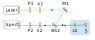
\includegraphics{../figures/setup_simplified.pdf}
	\caption{Used setup for photoluminescence measurements.}
	\label{fig:pl setup}
\end{figure}
A setup to measure polarization-sensitive photoluminescence is illustrated in \autoref{fig:pl setup}.

The excitation laser at \SI{532}{nm} or \SI{647}{nm} is polarization-controlled using the polarizer P$_1$ and the retarder $\lambda_1$.\\
The mirror M$_1$ with the beam splitter BS$_2$ is located at a small angle to preserve the polarization as much as possible.
The beam splitter BS$_2$ is a polka dot mirror because it minimizes the changes in polarization compared to a glass wedge.\\
The analysation path to the spectrometer is also polarization controlled with the retarder $\lambda_2$ and the polarizer P$_2$.

The retarders were configured to excite with circular polarization and detect with linear polarization or vice versa to prevent any bias in the excitation.\\
While this may not be necessary given that the excitation polarization is lost in the complex luminescence process \cite{NiPS3_linear}, it is a good practice to ensure that the measurements are not biased.

\begin{figure}
	\centering
	\includegraphics{../figures/2023-12-10 Combined PL.pdf}
	\caption{Measured Photoluminescence spectra at \SI{10}{K}.}
	\label{fig:pl}
\end{figure}
\autoref{fig:pl} depicts the photoluminescence spectra of various samples at \SI{10}{K}.
This is selected as the peaks get sharper with decreasing temperature.\\
A main peak is observed, with different widths for the different materials. 
This Peak is caused by the exciton photoluminescence process \cite{NiPS3_exciton,CrPS4_pl}.\\
Next to the main peak, multiple smaller peaks are visible.
These are more complex structures such as excitons in higher energy levels, charged excitons, or biexcitons \cite{CrPS4_pl, NiPS3_exciton,NiPS3_anisotropic, NiPS3_coherent}.\\
For this project, only the respective main peak is considered.

Despite exfoliation to remove the rough surface, no photoluminescence was detected for FePS$_3$ which is consistent with the findings reported in \cite{FePS3_pl}.

\begin{figure}
	\centering
	\begin{subfigure}{2.5in}
		\includegraphics{../figures/2024-04-06 NiPS3 excitation power dependence.pdf}
		\caption{NiPS$_3$}
	\end{subfigure}
	\begin{subfigure}{2.5in}
		\includegraphics{../figures/2023-12-14 CrPS4 excitation power dependence.pdf}
		\caption{CrPS$_4$}
	\end{subfigure}
	\caption{Excitation power dependence of the photoluminescence signal at \SI{10}{K}.}
	\label{fig:pl power dependence spectra}
\end{figure}
It is standard practice to use an excitation power in the range of \SI{5}{uW} to \SI{5}{mW} to prevent damage to the sample \cite{NiPS3_anisotropic, NiPS3_exciton}.\\
However, the damage threshold is dependent on the power density, and neither the beam size nor the damage threshold is known.
In order to get an understanding of the saturation of the sample the power scaling was measured.\\
The resulting spectra for different excitation powers are shown in \autoref{fig:pl power dependence spectra}.
No unexpected drastic changes that would indicate damage to the sample are visible.\\

\begin{figure}
	\centering
	\includegraphics{../figures/2024-04-19 excitation power dependence of main pl line.pdf}
	\caption{Excitation power dependence of the main photoluminescence line at \SI{10}{K} with a quadratic and power law fit. }
	\label{fig:pl power dependence}
\end{figure}
To gain a more comprehensive understanding, the main peak can be integrated.
This is shown relative to the excitation power in \autoref{fig:pl power dependence}.

For NiPS$_3$, a quadratic function fitting indicates a linear scaling that begins to saturate at higher excitation powers.\\
For CrPS$_4$, the scaling is faster than linear, which can be explained by a scaling probability of creating biexcitons additionally to the exciton photoluminescence process \cite{biexciton}. \\
Since a power law fit is commonly used to describe the scaling the fit is also shown.

In order to achieve a good signal-to-noise ratio while avoiding saturating the sample, the excitation power was selected to be in the range of \SI{1}{mW} to \SI{4}{mW}.\\
Even when illuminated with \SI{20}{mW}, the sample did not exhibit any signs of damage.

However, following multiple measurements, the photoluminescence ceased in some NiPS$_3$ flakes.\\
This is not due to the excitation, as this also occurred in flakes that were not excited.
It is caused by oxidation during storage and manipulation of the samples.\\
There were no visible changes to those samples on optical microscope images.


\section{Measurement Setup}
\begin{figure}
	\centering
	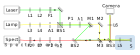
\includegraphics{../figures/setup.pdf}
	\caption{Full schematic at the end of the measurements.}
	\label{fig:schematic full}
\end{figure}
Upon completion of the measurements, the optical table had a few additional components not depicted on the simplified schematic \autoref{fig:pl setup}.
The full schematic is presented in \autoref{fig:schematic full}.

The sample $S$ could be illuminated with a fiber-coupled array of diode lasers, a fiber-coupled halogen lamp, and subsequently a white LED.
The lenses $L_{1-4}$ were used to expand the cross-section in order to utilize the entire size of $L_5$. \\
$F_1$ was a film filter used to block out the detection wavelengths from the excitation light.
Additionally, it creates a sharper spectral edge on the laser line for Raman spectroscopy.\\
The aperture $A_1$ was mounted off-center to illuminate the sample in a dark-field configuration, thereby increasing the contrast in the camera image.
Thanks to \textit{Mateusz Raczyński} for showing me this trick.\\
These two illumination paths were combined with cube beam splitters BS$_1$.
The polarizer P$_1$ and the retarder $\lambda_1$ were used to control the polarization of the light.\\
Then the mirror $M_1$ and the beam splitter BS$_2$ were used to introduce the light into the detection path without changing the polarization too much.\\
To get more light for the camera $M_1$ could be flipped out and $M_3$ could be flipped in.
This obstructs the spectrometer and compromises the polarization of the light, but increases the intensity by a factor of two.\\
$BS_3$ was just used to image the sample with the camera. 
It was a film beam splitter with a large aperture that has to be removed for polarization-sensitive measurements, as it is strongly polarizing.

The objective lens $L_5$ was on an x-y-z piezo stage in the cryostat to move and focus on different flakes of the sample.\\
The cryostat and the magnet are combined in a single unit since the \SI{10}{T} superconducting magnet needs a helium reservoir.
The sample was in a variable temperature insert (VTI) with a controllable helium cooling flow and a electric heater.
The magnet has metal heat shields in the vacuum isolation layer and a nitrogen jacket to isolate it even more.
Both isolation methods had problems:\\
The metal heat shield was bent on the magnet that was supposed to be used for the measurements.
This bridged the nitrogen and helium reservoir, which caused the helium to boil off pretty quickly.
But only when the VTI was cooled down, due to thermal contraction.\\
At the end of the measurements, somebody forgot to renew the contract with the company delivering the nitrogen, but they still delivered to the end of my measurements.

The light from the sample then goes through the retarder $\lambda_2$ and the polarizer P$_2$ to control the analysed polarization.\\
The retarder $\lambda_2$ was mounted on a computer-controlled rotation stage and connected to the PyLUMS software stack originally developed by \textit{Tomasz Kazimierczuk}, who was also of great help in solving numerous technical problems.

The light then was focused by the lens $L_7$ into the spectrometer.
$L_7$ had a focal length of \SI{20}{cm} arbitrarily chosen by the previous user.\\
The interference filter $F_2$ was used to block out the excitation light from the spectrometer and is placed as close to the spectrometer as possible to block out all the stray excitation light.

For Raman measurements, the filter was tuned by rotating it to change the effective thickness of the interference film.
\textit{Jan Suffczyński} helped to set up the Raman measurements, as he has measured it on NiPS$_3$ before. 

The used spectrometer was a \textit{ANDOR SR-500i} with a piezo-cooled CCD sensor and a 1200 lines/mm grating.


\chapter{Results}
With a suitable measurement technique established and a reliable setup in place, the optical signatures to probe the magnetic field could be identified.

\section{NiPS$_3$ Splitting and Rotation}
\begin{figure}
	\centering
	\includegraphics{../figures/2024-04-10 NiPS4 splitting.pdf}
	\caption{Different Splitting of the Photoluminescence line in NiPS$_3$ for different polarization direction at \SI{5}{K}.}
	\label{fig:NiPS3 splitting}
\end{figure}
First NiPS$_3$ was investigated due to the sharp photoluminescence line.
This was done with exfoliated flakes on a Si/SiO$_2$ substrate for easier handling.

As illustrated in \autoref{fig:NiPS3 splitting}, the line splits into two lines at higher fields.\\
The splitting $\Delta E$ is different for different polarization directions.
In the polarization direction where the external magnetic field is aligned with the electric field of the photoluminescence signal, the splitting $\Delta E$ is larger than in the perpendicular direction.

\begin{figure}
	\begin{subfigure}[t]{3.5in}
		\includegraphics{../figures/2024-04-21 NiPS3 DeltaE.pdf}
		\caption{$\Delta E$ mesuered with Bigaussian fit.}
		\label{fig:NiPS3 delta E}
	\end{subfigure}
	\begin{subfigure}[t]{2.5in}
		\includegraphics{../figures/2024-04-21 NiPS3 single polarisation.pdf}
		\caption{Recorded data for \SI{0}{\degree} with $\Delta E$ from \autoref{eq:NiPS3 model} }
		\label{fig:NiPS3 model}
	\end{subfigure}
	\caption{}
\end{figure}
To directly determine $\Delta E$ the sum of two Gaussian peaks was fitted, centered at $E\pm \nicefrac{\Delta E}{2}$ with the same amplitude $I$ and width $\sigma$.\\
$\sigma$ was fixed at a constant value as it is primarily dependent on the focus of the spectrometer \autocite{NiPS3_magnon_gap}.
$E$ and $I$ were fitted independently for each measurement over field and polarization angle, as the turning retarder and the field-dependent moving sample holder altered the position of the focus on the spectrometer and the focus on the sample, thereby changing $E$ and $I$ respectively.\\
\autoref{fig:NiPS3 delta E} depicts $\Delta E$ over the field and angle.

My supervisor \textit{Mateusz Goryca} found a publication in which the splitting was already documented \autocite{NiPS3_magnon_gap}.
Additionally, the authors proposed a mean-field biaxial antiferromagnet model that fits their data:\\
This model defines the angle $\psi$ between the spin of the $Ni^{2+}$-ions and the external magnetic field $\vec{H}$.
For $H=0$ the spin aligns with the $a$-crystal axis, and thus, the initial angle $\theta_0=\psi\left(H=0\right)=\measuredangle\left(a, H\right)$ can be defined.\\
The coupling constants along the axis of the model reduce to an effective $g$ factor and a spin-flop field $H_\text{sf}$. 
Consequently, the proposed model \autocite{NiPS3_magnon_gap} yields the following results:
\begin{align}
	\tan 2\psi &= \frac{\sin 2\theta_0}{\cos 2\theta_0 - \frac{H}{H_\text{SF}}^2}\\
	\Delta E &= \mu_B g H \cos \psi
	\label{eq:NiPS3 model}
\end{align}
This model does not include polarization-resolved differences as $\Delta E$ is independent of the polarization angle.
This is not observed in \autoref{fig:NiPS3 delta E}.\\
Nevertheless, by selecting a single polarization the model fits the data, as shown in \autoref{fig:NiPS3 model}.
Even the $g$-factor and the $H_\text{sf}$ are the same as in \autocite{NiPS3_magnon_gap}.

\begin{figure}
	\centering
	\begin{subfigure}{4in}
		\includegraphics{../figures/2024-04-18 NiPS4 splitting 10K.pdf}
		\caption{10K}
		\label{fig:NiPS3 10K}
	\end{subfigure}
	\begin{subfigure}{4in}
		\includegraphics{../figures/2024-04-18 NiPS4 splitting 10K multiple flakes.pdf}
		\caption{10K with multiple flakes}
		\label{fig:NiPS3 10K multiple flakes}
	\end{subfigure}
	\begin{subfigure}{4in}
		\includegraphics{../figures/2024-04-18 NiPS4 splitting 50K.pdf}
		\caption{50K}
	\end{subfigure}
	\caption{Splitting of the NiPS$_3$ photoluminescence line at different temperatures on different Flakes.}
	\label{fig:NiPS3 multiple temperatures}
\end{figure}
The splitting is most visible at low temperatures due to the narrower lines.
\autoref{fig:NiPS3 multiple temperatures} shows the same measurement at different Temperatures and for different samples.\\
At Temperatures above \SI{50}{K} the photoluminescence could not be reliably measured over the field, and thus the phase transition to paramagnetic at the Néel temperature of \SI{155}{K} \cite{MPS_magnetism} can not be observed.

In \autoref{fig:NiPS3 10K} and \autoref{fig:NiPS3 10K multiple flakes} the splitting is visible for different flakes at \SI{10}{K}.\\
\autoref{fig:NiPS3 10K multiple flakes} appears to show multiple overlaid splitting curves,
which can be explained by the model assuming that the crystal is broken into two different distinct orientations with different $\theta_0$, resulting in distinct splitting curves combined in the measurement.

Furthermore, the splitting and polarization dependence exhibit no hysteresis.


\begin{figure}
	\centering
	\includegraphics{../figures/2024-04-07 NiPS3 polarisation.pdf}
	\caption{Alignment of the polarization axis of the main photoluminescence line perpendicular to the external magnetic field at \SI{0}{\degree}.}
	\label{fig:NiPS3 polarisation peanut}
\end{figure}
Another publication \cite{NiPS3_linear} found that the linear polarization of the photoluminescence signal rotates to be perpendicular to the magnetic field. 
This phenomenon is illustrated in \autoref{fig:NiPS3 polarisation peanut}, which depicts the main peak of the photoluminescence signal measured with different polarisation angles to the magnetic field and a $cos^2$ fit. The peak was integrated from \SIrange{839}{841}{nm}.\\
This could suggest that the polarization of the entire peak just rotates.

\begin{figure}
	\centering
	\includegraphics{../figures/2024-04-09 NiPS3 polarisation Splitting.pdf}
	\caption{Results from the $\cos^2$ fit spectral resolved at \SI{5}{K}.}
	\label{fig:NiPS3 polarisation splitting}
\end{figure}
However, for the purpose of examining the polarization direction, the data presented in \autoref{fig:NiPS3 splitting} can be displayed differently.
By fitting the $\cos^2$ function for every wavelength and field individually the average intensity, polarization angle, and degree can be extracted, as shown in \autoref{fig:NiPS3 polarisation splitting}.

The line splits less when $P\perp H$ than when $P\parallel H$.\\
In the $\measuredangle P, H$-panel this is evident as a rotation of the polarization axis in the center of the photoluminescence line, that rotates from $\theta_0\approx \SI{30}{degree}$ to \SI{90}{degree}.\\
Bellow the edges of the split line, the polarization is parallel to the magnetic field, resulting in an angle of \SI{0}{degree}.
In between there is a visible line where the angle is \SI{45}{degree}.\\
This simplifies the interpretation of the data, as two images are combined into one.

In order to quantify the degree of polarization, it is necessary to define a reference level.
The background level was selected as the photoluminescence signal next to the peak, evaluated as the mean between \SIrange{845}{860}{nm}.

% The polarization of the main photoluminescence peak was measured as near unity in \cite{NiPS3_anisotropic}.
% However, the degree of polarization is only around \SI{0.5}{} in the presented data.\\
% This discrepancy may be due to the different excitation powers used in the measurements as they used \SI{5}{uW} compared to \SI{1}{mW} in this measurement.\\
% However it is hard to compare as they did not specify their reference level.

The measurement of polarized photoluminescence shows that the luminescence process is more complex than previously understood and more theoretical work is needed to explain it fully.

\clearpage

\section{CrPS$_4$ Circular Dichroism}
CrPS4 was examined next, as the photoluminescence behavior under a magnetic field was not yet documented.
The photoluminescence signal in CrPS$_4$ exhibited a notably stronger and broader profile compared to NiPS3.
No observable splitting or displacement of the peak in the photoluminescence signal was detected in response to changes in the magnetic field. 
Furthermore, while the photoluminescence signal in CrPS$_4$ displayed stronger linear polarization than in NiPS3, no rotational behavior attributable to the external magnetic field was observed.

\begin{figure}
	\begin{subfigure}[t]{3.5in}
		\includegraphics{../figures/2023-12-14 CrPS4 circular dichroism.pdf}
		\caption{Circular dichroism of the photoluminescence in CrPS$_4$.}
		\label{fig:CrPS4 CD}
	\end{subfigure}
	\begin{subfigure}[t]{2.5in}
		\includegraphics{CrPS4_magneto_tourque.pdf}
		\caption{Magnetisation measured using magneto torque from \cite{CrPS4_magnetic}.}
		\label{fig:CrPS4 magnetic}
	\end{subfigure}
	\caption{Comparison of circular dichroism of the photoluminescence line and the magnetization in CrPS$_4$.}
\end{figure}
Upon examination of the circular dichroism of the photoluminescence in CrPS$_4$ in \autoref{fig:CrPS4 CD},
a clear non-hysterical change over the magnetic field is evident.\\
This aligns perfectly with magneto torque measurements of the magnetization \autoref{fig:CrPS4 magnetic} from \cite{CrPS4_magnetic} in all measured magnetic field configurations and temperatures.
However, the corresponding authors have thus far refused to provide their data for quantitate comparison.\\
But at least from qualitative comparison, the circular dichroism of the photoluminescence line is proportional to the magnetization in CrPS$_4$. 

The circular dichroism is evaluated by integrating over the entire photoluminescence from \SIrange{890}{970}{nm}.
This reduces noise and is necessary to measure such small differences with the spectrometer.
However, there is no significant difference in the circular dichroism over the wavelength, so the spectrometer is not necessary.\\
The selection of the zero level for calculating the dichroism is obvious, as there is no significant different if it is taken sufficiently far away from the photoluminescence peak or with the excitation laser deactivated.

The circular dichroism-based magnetization measurement enables the identification of the spin-flop transition at \SI{.8}{T} and the spin-flip phase transition at \SI{7.5}{T}, which are discernible as distinct changes in the magnetization curve in \autoref{fig:CrPS4 CD}.
These transitions are characterized by \cite{CrPS4_magnetic}. 

But the method is not yet suitable for absolute magnetization measurement, as the circular dichroism to magnetization ratio differs between flakes.
This might depend on the thickness of the flakes.\\
But even without absolute measurements, the method is still useful, as it allows for fast and localized measurement of the magnetisation in CrPS$_4$, that were not possible with previous methods.

% \begin{figure}
% 	\centering
% 	\includegraphics{../figures/2024-04-10 susceptibility dichroism measurement.pdf}
% 	\caption{Susceptibility as the derivative of the measured circular dichroism signal.}
% 	\label{fig:CrPS4 susceptibility}
% \end{figure}
% As an example of the utility of the circular dichroism based measurement, \autoref{fig:CrPS4 susceptibility} depicts the susceptibility.
% This is calculated from the measured magnetization by taking the first derivative.

% This allows to easy locate the spin-flop transition at \SI{1}{T} and the spin-flip transition at \SI{7.5}{T}. 
% As characterized by \cite{CrPS4_magnetic}. 

\begin{figure}
	\centering
	\includegraphics{../figures/2024-04-22 CrPS4 temperature series.pdf}
	\caption{Photoluminescence for different temperatures.}
	\label{fig:CrPS4 temperature}
\end{figure}
The photoluminescence signal is still visible at room-temperature in \autoref{fig:CrPS4 temperature} and the phase transitions to paramagnetic at the Néel temperature of \SI{38}{K} \cite{CrPS4_magnetic} can be observed.\\
Therefore this method allows to study of the entire magnetic phase diagram of CrPS$_4$.


\clearpage
\subsection{Aligning Flakes}
\label{sec:aligning flakes}
\begin{figure}
	\begin{subfigure}{2.5in}
		\includegraphics{../figures/2024-01-23 rotating pl.pdf}
		\caption{First successful measurement.}
		\label{fig:alignment first}
	\end{subfigure}
	\begin{subfigure}{3.5in}
		\includegraphics{../figures/2024-01-29 rotating pl.pdf}
		\caption{Partially reproduced measurement on different substrates.}
		\label{fig:alignment second}
	\end{subfigure}
	\caption{Rotation of the linear polarization of the photoluminescence signal in CrPS$_4$ during cooling.}
	\label{fig:alignment}
\end{figure}
After a few days of measurements on CrPS$_4$, the linear polarization of the photoluminescence signal from all the flakes was aligned in the same direction.
This is unexpected for out-of-plane magnetic field measurements, as there was assumed to be no inherent axis in the plane and therefore symmetry for the in-plane rotational degree of freedom.

This was measured more systematically by creating new samples without any alignment in the exfoliation process.
For this, the adhesive tapes were rotated to arbitrary angles at each subdivision step and the transfer step was performed multiple times at different angles.

Then the linear polarization of a number of flakes was recorded during the cooling process, with particular care taken to ensure that no bias for one axis was introduced in the measurement.
Images were taken at each temperature in order to determine if the entire flake rotated or just the photoluminescence signal. 

The initial measurement \autoref{fig:alignment first} confirmed that the photoluminescence of all recorded flakes, which where randomly oriented at room-temperature, aligned to a single orientation at temperatures around \SI{200}{K}.
In the images no rotation of the flakes were observed.

It was suspected that the Si lattice of the Si/SiO$_2$ substrate introduces an alignment direction.
Therefore, a glass substrate was used, which should not have a preferred axis.  
The results are presented in \autoref{fig:alignment second}, along with a new Si/SiO$_2$ sample to reproduce the aforementioned result.\\
However, in this experiment not all flakes aligned, which indicates a significant variance in the sample preparation.\\
Nevertheless, the alignment directions are different, indicating that the directionality is not from the experimental setup.

The images of the flakes show no correlation between the alignment and the shape or size of the flakes. 
Furthermore, the alignment does not correlate with the distance to neighboring flakes or the substrate material.

\begin{figure}
	\centering
	\begin{subfigure}[t]{1.8in}
		\includegraphics{../figures/2024-04-19 AFM (a).pdf}
		\caption{Normal flake.}
		\label{fig:AFM normal}
	\end{subfigure}
	\begin{subfigure}[t]{1.8in}
		\includegraphics{../figures/2024-04-19 AFM (b).pdf}
		\caption{Thin, torn flake.}
		\label{fig:AFM torn}
	\end{subfigure}
	\begin{subfigure}[t]{1.8in}
		\includegraphics{../figures/2024-04-19 AFM (c).pdf}
		\caption{Flake with a rough surface.}
		\label{fig:AFM rough}
	\end{subfigure}
	\caption{Atomic force microscopy images of CrPS$_4$ flakes.}
	\label{fig:AFM}
\end{figure}
Following the measurements, \textit{Julia Kucharek} helped me to record atomic force microscopy images of the samples.\\
The flakes had a thickness ranging from \SIrange{200}{700}{nm}, as shown in \autoref{fig:AFM}.

In the case of the sample where all flakes aligned, all flakes had a smooth surface like in \autoref{fig:AFM normal} and \autoref{fig:AFM torn}.

On the samples where not all flakes aligned, some flakes had a rough surface, as shown in \autoref{fig:AFM rough}.
This rough patch extended over the flakes' boundary to the bare substrate.
This is likely residue from the adhesive used in the exfoliation process.

Additionally, thinner flakes on the Si/SIO$_2$ substrate had cracks in the surface as shown in \autoref{fig:AFM torn}.
The observed cracks appear to be mechanical stress fractures.
The origin of these cracks, whether due to unequal thermal expansion or from the mechanical exfoliation process, remains unclear. 



\chapter{Conclusion and Outlook}
Three and half months of measurements yielded a couple of interesting results:

The NiPS$_3$ polarized photoluminescence measurements serve as an additional data point for validating models of the luminescence process.
The luminescence is linearly polarized, exhibiting a distinct splitting for different polarization directions.\\
The objective now is to compare different models for the luminescence process \cite{NiPS3_coherent, MPX_first_principles} with the measurements. 

The CrPS$_4$ circular dichroism measurements represent a novel technique for probing the magnetization in this material.
This result will be directly utilized for further research into the magnetic properties of CrPS$_4$ due to its capacity for easy and sensitive measurements on a limited sample volume.\\
As of the time of writing, additional data is being recorded by the group in Warsaw to enhance the reliability of the results.

It is dissatisfying that the reason for the alignment of the CrPS$_4$ flakes was not found.\\
But the next steps are clear:\\
Taking atomic force microscopy images after exfoliation, to see if flakes are already torn,\\
changing the temperature at the transfer step during exfoliation to see a possible correlation with the rough surface to prove that the rough surface is glue residue,\\
Washing away the glue to prove that it has a stabilizing effect on the flakes,\\
and trying substrates with different thermal expansion coefficients to see if the alignment correlates. \\
But all of these steps need a statistical argument, which takes many samples and time that I did not have.
But maybe a future student can pick up where I left off.
Because an unknown rotational symmetry-breaking mechanism in the process of exfoliation or the measurement is interesting, as many arguments assume that symmetry.



\backmatter
\addcontentsline{toc}{chapter}{Bibliography}
\nocite{*}
\printbibliography

\section*{Data Availability}
All the recorded data and software used for the analysis and documentation are available at \url{https://github.com/leoole100/bachelorarbeit_public}.

% \appendix
% \chapter{Appendix}


\end{document}